\graphicspath{{imgs/}}

%===============================================================================
\chapter{Introduction}
%===============================================================================
%


%-------------------------------------------------------------------------------
\section{Our Contribution}
%
Our contributions are as follows. We validate that the foremost wireless
algorithm for the understanding of the lookaside buffer by O.  Moore
\cite{cite:0} is maximally efficient. Further, we explore new real-time
methodologies ({Hyp}), which we use to show that the little-known
knowledge-based algorithm for the exploration of the Turing machine by Taylor
et al. \cite{cite:0} runs in
%
\begin{equation}
	\Omega (\log \log \log {n} ^ { \log \log n })
	\label{eq:eq1}
\end{equation}
%
time. This outcome might seem unexpected but has ample historical precedence.

The rest of this paper is organized as follows. Primarily,  we motivate the
need for DNS. On a similar note, we disprove the refinement of 2 bit
architectures.  We place our work in context with the existing work in this
area. Ultimately, we conclude.

\thesisstructure Add here a brief description of the structure of the thesis.

%===============================================================================
\chapter{Principles}
%===============================================================================
%


\begin{figure}[htpb]
	\centering
	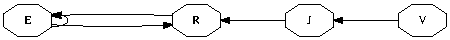
\includegraphics{dia0}
	\caption{%
	The relationship between our heuristic and the robust unification of
	local-area networks and congestion control.
	}
	\label{fig:introLabel0}
\end{figure}



\begin{equation}
	\mathcal{N} = \nabla\bcdot\boldsymbol{u}
	\label{eq:eq2}
\end{equation}


%-------------------------------------------------------------------------------
\section{Stochastic Technology}
%


%===============================================================================
\chapter{Evaluation}
%===============================================================================
%



%-------------------------------------------------------------------------------
\section{Hardware and Software Configuration}
%
\begin{figure}[htpb]
	\centering
	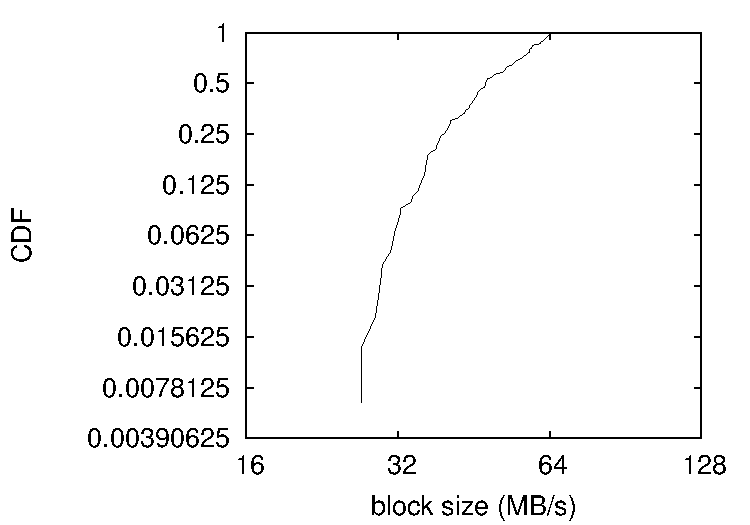
\includegraphics[width=0.7\textwidth]{figure0}
	\caption{%
	The median throughput of Hyp, as a function of bandwidth.
	}
	\label{fig:introLabel2}
\end{figure}



\begin{figure}[htpb]
	\centering
	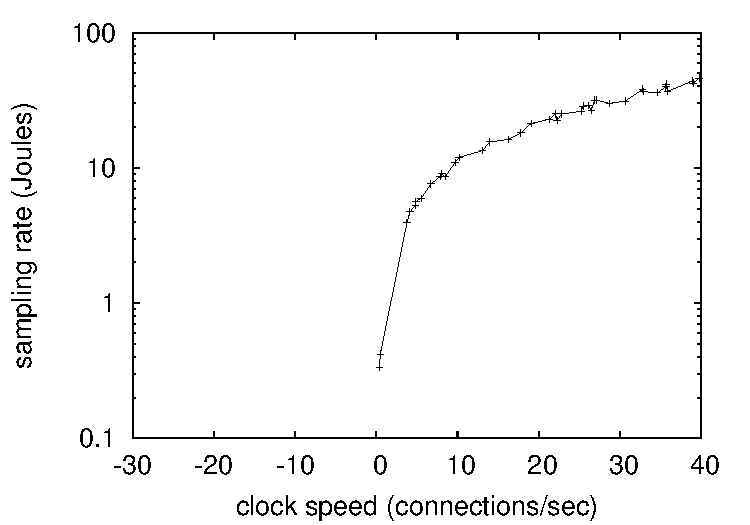
\includegraphics[width=0.7\textwidth]{figure1}
	\caption{%
	The median sampling rate of Hyp, as a function of energy.
	}
	\label{fig:introLabel3}
\end{figure}



\begin{figure}[htpb]
	\centering
	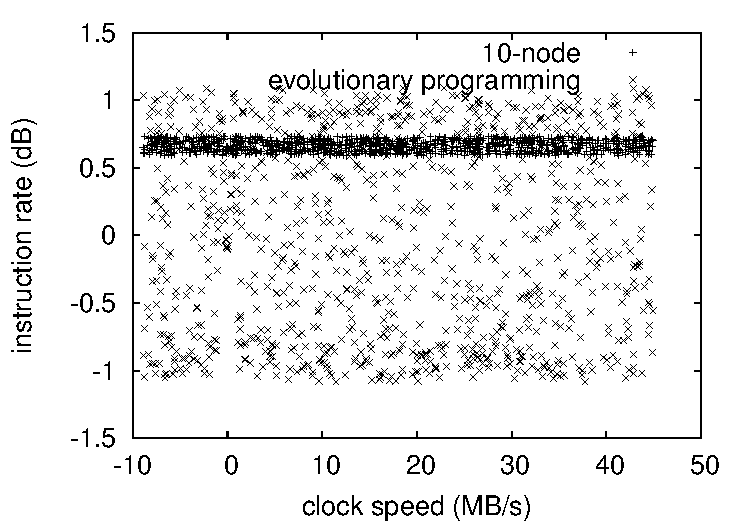
\includegraphics[width=0.7\textwidth]{figure2}
	\caption{%
	The expected energy of our methodology, compared with the other algorithms.
	}
	\label{fig:introLabel4}
\end{figure}


%-------------------------------------------------------------------------------
\section{Experimental Results}
%
\begin{figure}[htpb]
	\centering
	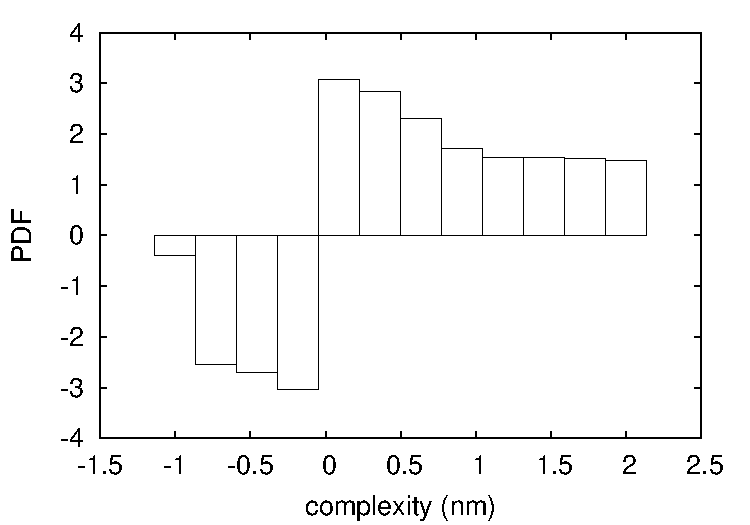
\includegraphics[width=0.7\textwidth]{figure3}
	\caption{
	These results were obtained by Y. Taylor et al. \cite{cite:3}; we reproduce
	them here for clarity. Of course, this is not always the case.
	}
	\label{fig:introLabel5}
\end{figure}






%===============================================================================
\chapter{Related Work}
%===============================================================================
%



%===============================================================================
\chapter{Conclusions and outlook}
%===============================================================================
%


%===============================================================================
\chapter{Test chapter, a very very very long title to test the table of contents}
%===============================================================================

This chapter is meant for testing the correct referencing of figures, equations
and tables.

% equations
%
\begin{equation}
	1 + 1 = 2
	\label{eq:test_eq1}
\end{equation}

\begin{align}
	2 + 2 = 4
	\label{eq:test_eq2}
\end{align}

\begin{equation}
	3 + 3 = 6
	\label{eq:test_eq3_intro}
\end{equation}

% tables
%
\begin{table}
	\centering
	\begin{tabular}{c}
		1
	\end{tabular}
	\caption{Test table 1}
	\label{tab:test_tab1}
\end{table}

\begin{table}
	\centering
	\begin{tabular}{c}
		2
	\end{tabular}
	\caption{Test table 2}
	\label{tab:test_tab2}
\end{table}

\begin{table}
	\centering
	\begin{tabular}{c}
		3
	\end{tabular}
	\caption{Test table 3}
	\label{tab:test_tab3_intro}
\end{table}

% figures
%
\begin{figure}[h!]
	\centering
	test figure 1
	\caption{Test figure 1}
	\label{fig:test_fig1}
\end{figure}

\begin{figure}[h!]
	\centering
	test figure 2
	\caption{Test figure 2}
	\label{fig:test_fig2}
\end{figure}

\begin{figure}[h!]
	\centering
	test figure 3
	\caption{Test figure 3}
	\label{fig:test_fig3_intro}
\end{figure}

% test references
%
\hrule
\begin{itemize}
	\item reference to equation 1: \eqref{eq:test_eq1}
	\item reference to equation 2: \eqref{eq:test_eq2}
	\item reference to equation 3: \eqref{eq:test_eq3_intro}
\end{itemize}
\hrule
\begin{itemize}
	\item reference to table 1: \eqref{tab:test_tab1}
	\item reference to table 2: \eqref{tab:test_tab2}
	\item reference to table 3: \eqref{tab:test_tab3_intro}
\end{itemize}
\hrule
\begin{itemize}
	\item reference to figure 1: \eqref{fig:test_fig1}
	\item reference to figure 2: \eqref{fig:test_fig2}
	\item reference to figure 3: \eqref{fig:test_fig3_intro}
\end{itemize}
\hrule

%===============================================================================
% Acknowledgments
%===============================================================================
%
\begin{acknowledgements}
%  Advisors,
%  funders,
%  collaborators,
%  mentors,
%  colleagues,
%  friends,
%  family.

  The first part of this thesis was written from December 2019 to January 2020, during the warmest winter since I arrived in Stockholm five years ago.
  Looking back, I have encountered, experienced and learned so much from uncountable people that is nearly impossible to name them one by one.
  I am grateful to \emph{everyone} and apologize in advance for any negligence.

  First and foremost, I thank Professor Luca Brandt for accepting me in and guiding me through the PhD program at KTH Mechanics.
  His strong leadership from the inception,
  enthusiastic responses and constructive criticisms at every discussion,
  generous support and increasing trust in me towards the end are indispensable for me to grow and develop academically.
  For these reasons, I owe my deepest gratitude to him.

  Second, I wish to extend my sincere thanks to my day-to-day advisors and mentors at KTH.
  I thank Outi Tammisolar for co-advising me since my first project, following my progress throughout the PhD
  and offering me invaluable career advice in the later years.
  I thank Jean-Christophe Loiseau for instilling in me the European culture, proper programming and mathematical rigour.
  I also thank Mehdi Niazi for always being available for technical discussions or code debugging and sharing his wisdom whenever I am lost.
  The patience, support and encouragement they offered me are instrumental in building my confidence and independence, which I will never take for granted.

  Third, I want to express my appreciation to all collaborators and senior colleagues that have shaped and contributed to my PhD work.
  These include, but are not limited to, international collaborators: Michael Dodd, Alexander Leshansky, Itzhak Fouxon and Naoki Takeishi;
  former and present colleagues at KTH: Walter Fornari, Pedro Costa, Francesco de Vita, Marco Rosti, B. M. Ningegowda and U\'{g}is L\={a}cis;
  office mates: Ricardo Vinuesa, Ekaterina Ezhova, Tímea Kékesi, Arash Alizad Banaei and Ashwin Vishnu;
  and professors that I enjoy talking to or playing innebandy with:
  Shervin Bagheri, Christophe Duwig, Hanno Essén, Nicholas Apazidis, Lanie Gutierrez-Farewik and Fredrik Lundell.
  Many others have also helped, corrected or inspired me in various research projects;
  my thanks are expressed in the separate acknowledgements after each paper in the next part of the thesis.
  
  In his famous essay, \emph{\small The World As I See It}, Einstein wrote,
  ``But from the point of view of daily life, without going deeper, we exist for our fellowmen --
  in the first place for those on whose smiles and welfare all our happiness depends,
  and next for all those unknown to us personally with whose destinies we are bound up by the tie of sympathy.''
  In the last several years, I have been lucky to derive plentiful happiness and sympathy from Artem, Erik, Guillaume, Nicolas, Frida, Natasha, Thea, Lee,
  as well as the rest of the Roslagstullsbacken corridor.
  Particularly, I am blessed to meet Dia, whose courage, ambition, curiosity and sensitivity have become a continuing source of my attachment,
  making me feel thorough and complete.
  
  Finally, none of the above would have been possible without the enduring love, hope, protection and education from my family at home.
  
  \chinese{爸,妈}
  
  \chinese{感谢你们对我从小到大的培养}

  \chinese{感谢你们对我的一切付出}

  \chinese{我的所有都属于你们}
  
  
\end{acknowledgements}



%===============================================================================
% References
%===============================================================================
%
\bibliographystyle{jfm}
\bibliography{thesis}
%
\IfFileExists{overview.bbl}{\graphicspath{{imgs/}}

%===============================================================================
\chapter{Introduction}
%===============================================================================



In \cite{Batchelor} we believe.


%-------------------------------------------------------------------------------

\section{Flow-assist droplet assembly}

material science,
photonic crystals,
microfluidics,
lab-on-a-chip.


\section{Liquid-infused surfaces}

drag reduction,
surface engineering,
superhydrophobicity,
lubricant-infused surfaces.


\section{Suspension flows}

particle suspensions,
complex fluids,
rheology,
shear thickening.

\thesisstructure Add here a brief description of the structure of the thesis.



%===============================================================================
\chapter{Microhydrodynamics}
%===============================================================================


In this chapter, we give a brief theoretical background of the topics studied.

mention the abuse of terms between droplets and particles.

The incompressible Navier-Stokes equation
\begin{subequations}
 \begin{equation}
   \nabla \cdot {\bm u} = 0,
  \label{eq:div-free}
 \end{equation}
 \begin{equation}
   \rho \bigg(\frac{\partial {\bm u}}{\partial t} + {\bm u} \cdot \nabla {\bm u} \bigg) = -\nabla p + \mu \nabla ^2  {\bm u} + {\bm f},
  \label{eq:NS}
 \end{equation}
\end{subequations}
governs the dynamics of Newtonian fluids (which is what we consider throughout the thesis).
where...

boundary conditions... between fluid and solid: continuity of the tangential velocity, \ie the no-slip condition (molecular slip ignored).
with an interface... surface tension... free surface... a boundary condition for the stress (see \cite{Batchelor} Sec.\ 3.3).


the Reynolds, Weber, and Froude numbers, defined as
\begin{equation}
  \begin{aligned}
    Re = \frac{\tilde{\rho} \tilde{U} \tilde{L}}{\tilde{\mu}},\quad \quad We = \frac{\tilde{\rho} \tilde{U}^2 \tilde{L}}{\tilde{\sigma}},\quad \quad Fr=\frac{\tilde{U}^2}{\tilde{g}\tilde{L}},      
  \label{eq:non-di-num}    
  \end{aligned}
\end{equation}
\noindent where $\tilde{U}$, $\tilde{L}$, $\tilde{\rho_1}$, $\tilde{\mu_1}$, and $\tilde{g}$ denote the reference dimensional velocity, length, density, dynamic viscosity, and gravitational acceleration. Note that $\rho_1=1$ and $\mu_1=1$ (i.e.\ we define fluid 1 as the reference fluid).
Perhaps also mention the Stouhal number.



%-------------------------------------------------------------------------------

\section{Stokes flow and its symmetries}

When small Reynolds number, Eq.\ \eqref{eq:NS} reduces to the Stokes equation,
\begin{equation}
   -\nabla p + \mu \nabla ^2  {\bm u} + {\bm f} = {\bm 0},
 \label{eq:Stokes}
\end{equation}
or, equivalently
\begin{equation}
   \nabla \cdot  {\bm \sigma} + {\bm f} = {\bm 0},
 \label{eq:Stokes1}
\end{equation}
where...

Stokes flow has the following symmetries and properties.
\begin{enumerate}
 \item \emph{Linearity}, which renders the applicability of superposition principle. For example, if $({\bm u}_1,p_1)$ is a solution to ${\bm f}={\bm f}_1$ and $({\bm u}_2,p_2)$ is a solution to ${\bm f}={\bm f}_2$, then $(\alpha{\bm u}_1+\beta {\bm u}_2,\alpha p_1 + \beta p_2)$ is a solution to ${\bm f}=\alpha{\bm f}_1 + \beta {\bm f}_2$.
 \item \emph{Reversibility}, which follows from the linearity and entails that, if the forcing changes from ${\bm f}$ to $-{\bm f}$, then the flow should reverse, \ie $({\bm u},p) \to (-{\bm u},-p)$. Note that, the simple reversibility symmetry can be very useful in deducing qualitative results without doing any calulation, see \eg the much celebrated note of \cite{Purcell1977}
 \item \emph{Stress equilibrium}, which states that any force exerted within the fluid is transmitted instantaneously to the boundary or, if there is no boundary, to infinity \citep{graham_2018}.
 \item \emph{Lorentz reciprocal relation}, which relates two solutions, $({\bm u}', {\bm \sigma}')$ and $({\bm u}'', {\bm \sigma}'')$ (they may differ by boundary conditions), of the Stokes equation by,
 \begin{equation}
  \small
  \begin{aligned}
   \int_V \bigg({\bm u}' \cdot (\nabla  \cdot {\bm \sigma}'') - {\bm u}'' \cdot (\nabla  \cdot {\bm \sigma}')\bigg) dV  & =\\
   \int_S \bigg({\bm u}' \cdot ({\bm n} \cdot {\bm \sigma}'') - {\bm u}'' \cdot ({\bm n} \cdot {\bm \sigma}')\bigg) dS, & 
  \end{aligned} \label{eq:lorentz-recip}
 \end{equation}
 where $V$ is some enclosed volume with surface $S$.
 \item \emph{Minimum dissipation principle}, which is a variational principle that asserts that the flow that minimizes energy dissipation rate subject to incompressibility and certain boundary conditions is the Stokes flow in that geometry.
\end{enumerate}


\section{Single particle in Stokes flow}

Green's function (Stoekslet),
stresslet (symmetric and traceless),
scaling laws (decay),
Fax\'{e}n's law,
confinement,
multipole expansion,
boundary integral methods.


\section{Particle interactions}

Batchelor and Green (1972),
swapping,
dancing,
range of interactions,
dipolar theory,
lubrication approximation.


\section{Rheology}

microstructure,
many-body problems (theoretical difficulties),
macroscopic properties, averages and bulk stresses (see Brady and Bossis).

The behaviour of systems involving the motion of small particles relative to a suspending fluid covers a wide range of phenomena of interest to both scientists and engineers. Dense suspensions, where the volume fraction of solid particles becomes comparable to or even higher than that of the fluid (see Figure \ref{fig:snap}), have particularly rich and sometimes unexpected rheologies, such as yielding, shear thinning, continuous shear thickening (CST), or discontinuous shear thickening (DST) \citep{mewis_wagner_book, Morton_Morris_2014, guazzelli_pouliquen_2018, Morris_annurev2020}. Apart from being theoretically intriguing, these complex behaviours often have major implications in practice. For instance, while it makes sense for the cement industry to manufacture suspensions that do not shear thicken, the same feature becomes an advantage for designing flexible body armor.



%===============================================================================
\chapter{Numerical Methods}
%===============================================================================



limitation of theoretical approaches,
necessity of numerical solutions.

Despite the practical importance, theoretical development of suspension rheology remains chanllenging and only a few analytical solutions have been found in the dilute regime, see \eg \cite{Einstein_1906, batchelor_green_1972b}. This is partially due to a lack of precise knowledge or control of various interactions at the particle level, partially due to the mathematical difficulties involved in many-body problems. On the other hand, solving a system of interacting particles is relatively straightforward in an algorithmic perspective. In fact, the last decades have seen tremendous advancement in both numerical simulations and computer hardware.

governing equations.

numerical solutions.


%-------------------------------------------------------------------------------

\section{Fluid-resolved methods}

level set methods,
(interface-correction level set/ghost fluid method),
volume-of-fluid methods,
phase-field methods,
immersed boundary methods.


\section{Particle-based methods}

The central equation to solve is
\begin{equation} 
 \begin{aligned} \label{eq:force-balance}
  {\bm m} \cdot \frac{d{\bm U}}{dt} = {\bm F}^H + {\bm F}^P, 
 \end{aligned}
\end{equation}
where ${\bm m}$ is a generalized mass/moment-of-inertia matrix of dimension $6N \times 6N$,
${\bm U}$ is the particle translational/rotational velocity vector of dimension $6N$,
and ${\bm F}$ represent the $6N$ force/torque vectors owing to hydrodynamics (denoted with superscript $\footnotesize H$) or other interactions (denoted with superscript $\footnotesize P$). Specifically, ${\bm F}^P$ may include contact, electrostatic, van der Waars, or magnetic forces, \etc. In principle, stochastic forces can also be included in the general formulation, though its numerical treatments demand special care such that fluctuation-dissipation theorem is satified. In the present thesis, Brownian motions are neglected.

For inertialess particles in Stokes flow, the task is to solve Eq.\ \eqref{eq:force-balance} subject to ${\bm m} \cdot (d{\bm U}/dt) \to 0$. Various techniques exist as summarized below.

\subsection{Stokesian dynamics}

The Stokesian dynamics \citep{Brady_Bossis1988} employs the fact that, when the particle Reynolds number is small and the bulk flow is linear, the hydrodynamic forces and stresses exerted on the particles by the fluid can be expressed as
\begin{equation} 
 \begin{aligned} \label{eq:sd-hydro}
  \begin{pmatrix}
   {\bm F}^H \\
   {\bm S}^H
  \end{pmatrix}
  = - \mathscr{R} \cdot
  \begin{pmatrix}
   {\bm U}-{\bm U}^\infty \\
   -{\bm E}^\infty
  \end{pmatrix},
 \end{aligned}
\end{equation}
where
\begin{equation} 
 \begin{aligned}
  \mathscr{R} =
  \begin{pmatrix}
   {\bm R}_{FU} & {\bm R}_{FE} \\
   {\bm R}_{SU} & {\bm R}_{SE}
  \end{pmatrix},
 \end{aligned}
\end{equation}
is termed the ``grand resistance'' matrix. 
If $\mathscr{R}$ is known, 
formulate the problem as

It is calculated as
\begin{equation} 
 \begin{aligned}
  \mathscr{R} = (\mathscr{M}^\infty)^{-1} +\mathscr{R}_{2B} - \mathscr{R}_{2B}^\infty.
 \end{aligned}
\end{equation}          
Es.\ \eqref{eq:sd-hydro} is then inverted and integrated in time to obtain the dynamics.


\subsection{Dissipative particle dynamics}

dissipative particle dynamics (DPD) \citep{Hoogerbrugge_1992, Groot_Warren_1997}


\subsection{Discrete element methods}


discrete element methods (DEM) \citep{Mari_Seto_2014JoR, Cheal_Ness_2018}, to name a few.
 the discrete-element lubrication/contact dynamics (DLCD) model.




%===============================================================================
\chapter{Summary}
%===============================================================================






%%===============================================================================
%\chapter{Test chapter, a very very very long title to test the table of contents}
%%===============================================================================
%
%This chapter is meant for testing the correct referencing of figures, equations
%and tables.
%
%% equations
%%
%\begin{equation}
%	1 + 1 = 2
%	\label{eq:test_eq1}
%\end{equation}
%
%\begin{align}
%	2 + 2 = 4
%	\label{eq:test_eq2}
%\end{align}
%
%\begin{equation}
%	3 + 3 = 6
%	\label{eq:test_eq3_intro}
%\end{equation}
%
%% tables
%%
%\begin{table}
%	\centering
%	\begin{tabular}{c}
%		1
%	\end{tabular}
%	\caption{Test table 1}
%	\label{tab:test_tab1}
%\end{table}
%
%\begin{table}
%	\centering
%	\begin{tabular}{c}
%		2
%	\end{tabular}
%	\caption{Test table 2}
%	\label{tab:test_tab2}
%\end{table}
%
%\begin{table}
%	\centering
%	\begin{tabular}{c}
%		3
%	\end{tabular}
%	\caption{Test table 3}
%	\label{tab:test_tab3_intro}
%\end{table}
%
%% figures
%%
%\begin{figure}[h!]
%	\centering
%	test figure 1
%	\caption{Test figure 1}
%	\label{fig:test_fig1}
%\end{figure}
%
%\begin{figure}[h!]
%	\centering
%	test figure 2
%	\caption{Test figure 2}
%	\label{fig:test_fig2}
%\end{figure}
%
%\begin{figure}[h!]
%	\centering
%	test figure 3
%	\caption{Test figure 3}
%	\label{fig:test_fig3_intro}
%\end{figure}
%
%% test references
%%
%\hrule
%\begin{itemize}
%	\item reference to equation 1: \eqref{eq:test_eq1}
%	\item reference to equation 2: \eqref{eq:test_eq2}
%	\item reference to equation 3: \eqref{eq:test_eq3_intro}
%\end{itemize}
%\hrule
%\begin{itemize}
%	\item reference to table 1: \eqref{tab:test_tab1}
%	\item reference to table 2: \eqref{tab:test_tab2}
%	\item reference to table 3: \eqref{tab:test_tab3_intro}
%\end{itemize}
%\hrule
%\begin{itemize}
%	\item reference to figure 1: \eqref{fig:test_fig1}
%	\item reference to figure 2: \eqref{fig:test_fig2}
%	\item reference to figure 3: \eqref{fig:test_fig3_intro}
%\end{itemize}
%\hrule

%===============================================================================
% Acknowledgments
%===============================================================================
%
\begin{acknowledgements}
%  Advisors,
%  funders,
%  collaborators,
%  mentors,
%  colleagues,
%  friends,
%  family.

  The first part of this thesis was written from December 2019 to January 2020, during the warmest winter since I arrived in Stockholm five years ago.
  Looking back, I have encountered, experienced and learned so much from uncountable people that is nearly impossible to name them one by one.
  I am grateful to \emph{everyone} and apologize in advance for any negligence.

  First and foremost, I thank Professor Luca Brandt for accepting me in and guiding me through the PhD program at KTH Mechanics.
  His strong leadership from the inception,
  enthusiastic responses and constructive criticisms at every discussion,
  generous support and increasing trust in me towards the end are indispensable for me to grow and develop academically.
  For these reasons, I owe my deepest gratitude to him.

  Second, I wish to extend my sincere thanks to my day-to-day advisors and mentors at KTH.
  I thank Outi Tammisolar for co-advising me since my first project, following my progress throughout the PhD
  and offering me invaluable career advice in the later years.
  I thank Jean-Christophe Loiseau for instilling in me the European culture, proper programming and mathematical rigour.
  I also thank Mehdi Niazi for always being available for technical discussions or code debugging and sharing his wisdom whenever I am lost.
  The patience, support and encouragement they offered me are instrumental in building my confidence and independence, which I will never take for granted.

  Third, I want to express my appreciation to all collaborators and senior colleagues that have shaped and contributed to my PhD work.
  These include, but are not limited to, international collaborators: Michael Dodd, Alexander Leshansky, Itzhak Fouxon and Naoki Takeishi;
  former and present colleagues at KTH: Walter Fornari, Pedro Costa, Francesco de Vita, Marco Rosti, B. M. Ningegowda and U\'{g}is L\={a}cis;
  office mates: Ricardo Vinuesa, Ekaterina Ezhova, Tímea Kékesi, Arash Alizad Banaei and Ashwin Vishnu;
  and professors that I enjoy talking to or playing innebandy with:
  Shervin Bagheri, Christophe Duwig, Hanno Essén, Nicholas Apazidis, Lanie Gutierrez-Farewik and Fredrik Lundell.
  Many others have also helped, corrected or inspired me in various research projects;
  my thanks are expressed in the separate acknowledgements after each paper in the next part of the thesis.
  
  In his famous essay, \emph{\small The World As I See It}, Einstein wrote,
  ``But from the point of view of daily life, without going deeper, we exist for our fellowmen --
  in the first place for those on whose smiles and welfare all our happiness depends,
  and next for all those unknown to us personally with whose destinies we are bound up by the tie of sympathy.''
  In the last several years, I have been lucky to derive plentiful happiness and sympathy from Artem, Erik, Guillaume, Nicolas, Frida, Natasha, Thea, Lee,
  as well as the rest of the Roslagstullsbacken corridor.
  Particularly, I am blessed to meet Dia, whose courage, ambition, curiosity and sensitivity have become a continuing source of my attachment,
  making me feel thorough and complete.
  
  Finally, none of the above would have been possible without the enduring love, hope, protection and education from my family at home.
  
  \chinese{爸,妈}
  
  \chinese{感谢你们对我从小到大的培养}

  \chinese{感谢你们对我的一切付出}

  \chinese{我的所有都属于你们}
  
  
\end{acknowledgements}



%===============================================================================
% References
%===============================================================================
%
\bibliographystyle{jfm}
\bibliography{thesis}
%
\IfFileExists{overview.bbl}{\graphicspath{{imgs/}}

%===============================================================================
\chapter{Introduction}
%===============================================================================



In \cite{Batchelor} we believe.


%-------------------------------------------------------------------------------

\section{Flow-assist droplet assembly}

material science,
photonic crystals,
microfluidics,
lab-on-a-chip.


\section{Liquid-infused surfaces}

drag reduction,
surface engineering,
superhydrophobicity,
lubricant-infused surfaces.


\section{Suspension flows}

particle suspensions,
complex fluids,
rheology,
shear thickening.

\thesisstructure Add here a brief description of the structure of the thesis.



%===============================================================================
\chapter{Microhydrodynamics}
%===============================================================================


In this chapter, we give a brief theoretical background of the topics studied.

mention the abuse of terms between droplets and particles.

The incompressible Navier-Stokes equation
\begin{subequations}
 \begin{equation}
   \nabla \cdot {\bm u} = 0,
  \label{eq:div-free}
 \end{equation}
 \begin{equation}
   \rho \bigg(\frac{\partial {\bm u}}{\partial t} + {\bm u} \cdot \nabla {\bm u} \bigg) = -\nabla p + \mu \nabla ^2  {\bm u} + {\bm f},
  \label{eq:NS}
 \end{equation}
\end{subequations}
governs the dynamics of Newtonian fluids (which is what we consider throughout the thesis).
where...

boundary conditions... between fluid and solid: continuity of the tangential velocity, \ie the no-slip condition (molecular slip ignored).
with an interface... surface tension... free surface... a boundary condition for the stress (see \cite{Batchelor} Sec.\ 3.3).


the Reynolds, Weber, and Froude numbers, defined as
\begin{equation}
  \begin{aligned}
    Re = \frac{\tilde{\rho} \tilde{U} \tilde{L}}{\tilde{\mu}},\quad \quad We = \frac{\tilde{\rho} \tilde{U}^2 \tilde{L}}{\tilde{\sigma}},\quad \quad Fr=\frac{\tilde{U}^2}{\tilde{g}\tilde{L}},      
  \label{eq:non-di-num}    
  \end{aligned}
\end{equation}
\noindent where $\tilde{U}$, $\tilde{L}$, $\tilde{\rho_1}$, $\tilde{\mu_1}$, and $\tilde{g}$ denote the reference dimensional velocity, length, density, dynamic viscosity, and gravitational acceleration. Note that $\rho_1=1$ and $\mu_1=1$ (i.e.\ we define fluid 1 as the reference fluid).
Perhaps also mention the Stouhal number.



%-------------------------------------------------------------------------------

\section{Stokes flow and its symmetries}

When small Reynolds number, Eq.\ \eqref{eq:NS} reduces to the Stokes equation,
\begin{equation}
   -\nabla p + \mu \nabla ^2  {\bm u} + {\bm f} = {\bm 0},
 \label{eq:Stokes}
\end{equation}
or, equivalently
\begin{equation}
   \nabla \cdot  {\bm \sigma} + {\bm f} = {\bm 0},
 \label{eq:Stokes1}
\end{equation}
where...

Stokes flow has the following symmetries and properties.
\begin{enumerate}
 \item \emph{Linearity}, which renders the applicability of superposition principle. For example, if $({\bm u}_1,p_1)$ is a solution to ${\bm f}={\bm f}_1$ and $({\bm u}_2,p_2)$ is a solution to ${\bm f}={\bm f}_2$, then $(\alpha{\bm u}_1+\beta {\bm u}_2,\alpha p_1 + \beta p_2)$ is a solution to ${\bm f}=\alpha{\bm f}_1 + \beta {\bm f}_2$.
 \item \emph{Reversibility}, which follows from the linearity and entails that, if the forcing changes from ${\bm f}$ to $-{\bm f}$, then the flow should reverse, \ie $({\bm u},p) \to (-{\bm u},-p)$. Note that, the simple reversibility symmetry can be very useful in deducing qualitative results without doing any calulation, see \eg the much celebrated note of \cite{Purcell1977}
 \item \emph{Stress equilibrium}, which states that any force exerted within the fluid is transmitted instantaneously to the boundary or, if there is no boundary, to infinity \citep{graham_2018}.
 \item \emph{Lorentz reciprocal relation}, which relates two solutions, $({\bm u}', {\bm \sigma}')$ and $({\bm u}'', {\bm \sigma}'')$ (they may differ by boundary conditions), of the Stokes equation by,
 \begin{equation}
  \small
  \begin{aligned}
   \int_V \bigg({\bm u}' \cdot (\nabla  \cdot {\bm \sigma}'') - {\bm u}'' \cdot (\nabla  \cdot {\bm \sigma}')\bigg) dV  & =\\
   \int_S \bigg({\bm u}' \cdot ({\bm n} \cdot {\bm \sigma}'') - {\bm u}'' \cdot ({\bm n} \cdot {\bm \sigma}')\bigg) dS, & 
  \end{aligned} \label{eq:lorentz-recip}
 \end{equation}
 where $V$ is some enclosed volume with surface $S$.
 \item \emph{Minimum dissipation principle}, which is a variational principle that asserts that the flow that minimizes energy dissipation rate subject to incompressibility and certain boundary conditions is the Stokes flow in that geometry.
\end{enumerate}


\section{Single particle in Stokes flow}

Green's function (Stoekslet),
stresslet (symmetric and traceless),
scaling laws (decay),
Fax\'{e}n's law,
confinement,
multipole expansion,
boundary integral methods.


\section{Particle interactions}

Batchelor and Green (1972),
swapping,
dancing,
range of interactions,
dipolar theory,
lubrication approximation.


\section{Rheology}

microstructure,
many-body problems (theoretical difficulties),
macroscopic properties, averages and bulk stresses (see Brady and Bossis).

The behaviour of systems involving the motion of small particles relative to a suspending fluid covers a wide range of phenomena of interest to both scientists and engineers. Dense suspensions, where the volume fraction of solid particles becomes comparable to or even higher than that of the fluid (see Figure \ref{fig:snap}), have particularly rich and sometimes unexpected rheologies, such as yielding, shear thinning, continuous shear thickening (CST), or discontinuous shear thickening (DST) \citep{mewis_wagner_book, Morton_Morris_2014, guazzelli_pouliquen_2018, Morris_annurev2020}. Apart from being theoretically intriguing, these complex behaviours often have major implications in practice. For instance, while it makes sense for the cement industry to manufacture suspensions that do not shear thicken, the same feature becomes an advantage for designing flexible body armor.



%===============================================================================
\chapter{Numerical Methods}
%===============================================================================



limitation of theoretical approaches,
necessity of numerical solutions.

Despite the practical importance, theoretical development of suspension rheology remains chanllenging and only a few analytical solutions have been found in the dilute regime, see \eg \cite{Einstein_1906, batchelor_green_1972b}. This is partially due to a lack of precise knowledge or control of various interactions at the particle level, partially due to the mathematical difficulties involved in many-body problems. On the other hand, solving a system of interacting particles is relatively straightforward in an algorithmic perspective. In fact, the last decades have seen tremendous advancement in both numerical simulations and computer hardware.

governing equations.

numerical solutions.


%-------------------------------------------------------------------------------

\section{Fluid-resolved methods}

level set methods,
(interface-correction level set/ghost fluid method),
volume-of-fluid methods,
phase-field methods,
immersed boundary methods.


\section{Particle-based methods}

The central equation to solve is
\begin{equation} 
 \begin{aligned} \label{eq:force-balance}
  {\bm m} \cdot \frac{d{\bm U}}{dt} = {\bm F}^H + {\bm F}^P, 
 \end{aligned}
\end{equation}
where ${\bm m}$ is a generalized mass/moment-of-inertia matrix of dimension $6N \times 6N$,
${\bm U}$ is the particle translational/rotational velocity vector of dimension $6N$,
and ${\bm F}$ represent the $6N$ force/torque vectors owing to hydrodynamics (denoted with superscript $\footnotesize H$) or other interactions (denoted with superscript $\footnotesize P$). Specifically, ${\bm F}^P$ may include contact, electrostatic, van der Waars, or magnetic forces, \etc. In principle, stochastic forces can also be included in the general formulation, though its numerical treatments demand special care such that fluctuation-dissipation theorem is satified. In the present thesis, Brownian motions are neglected.

For inertialess particles in Stokes flow, the task is to solve Eq.\ \eqref{eq:force-balance} subject to ${\bm m} \cdot (d{\bm U}/dt) \to 0$. Various techniques exist as summarized below.

\subsection{Stokesian dynamics}

The Stokesian dynamics \citep{Brady_Bossis1988} employs the fact that, when the particle Reynolds number is small and the bulk flow is linear, the hydrodynamic forces and stresses exerted on the particles by the fluid can be expressed as
\begin{equation} 
 \begin{aligned} \label{eq:sd-hydro}
  \begin{pmatrix}
   {\bm F}^H \\
   {\bm S}^H
  \end{pmatrix}
  = - \mathscr{R} \cdot
  \begin{pmatrix}
   {\bm U}-{\bm U}^\infty \\
   -{\bm E}^\infty
  \end{pmatrix},
 \end{aligned}
\end{equation}
where
\begin{equation} 
 \begin{aligned}
  \mathscr{R} =
  \begin{pmatrix}
   {\bm R}_{FU} & {\bm R}_{FE} \\
   {\bm R}_{SU} & {\bm R}_{SE}
  \end{pmatrix},
 \end{aligned}
\end{equation}
is termed the ``grand resistance'' matrix. 
If $\mathscr{R}$ is known, 
formulate the problem as

It is calculated as
\begin{equation} 
 \begin{aligned}
  \mathscr{R} = (\mathscr{M}^\infty)^{-1} +\mathscr{R}_{2B} - \mathscr{R}_{2B}^\infty.
 \end{aligned}
\end{equation}          
Es.\ \eqref{eq:sd-hydro} is then inverted and integrated in time to obtain the dynamics.


\subsection{Dissipative particle dynamics}

dissipative particle dynamics (DPD) \citep{Hoogerbrugge_1992, Groot_Warren_1997}


\subsection{Discrete element methods}


discrete element methods (DEM) \citep{Mari_Seto_2014JoR, Cheal_Ness_2018}, to name a few.
 the discrete-element lubrication/contact dynamics (DLCD) model.




%===============================================================================
\chapter{Summary}
%===============================================================================






%%===============================================================================
%\chapter{Test chapter, a very very very long title to test the table of contents}
%%===============================================================================
%
%This chapter is meant for testing the correct referencing of figures, equations
%and tables.
%
%% equations
%%
%\begin{equation}
%	1 + 1 = 2
%	\label{eq:test_eq1}
%\end{equation}
%
%\begin{align}
%	2 + 2 = 4
%	\label{eq:test_eq2}
%\end{align}
%
%\begin{equation}
%	3 + 3 = 6
%	\label{eq:test_eq3_intro}
%\end{equation}
%
%% tables
%%
%\begin{table}
%	\centering
%	\begin{tabular}{c}
%		1
%	\end{tabular}
%	\caption{Test table 1}
%	\label{tab:test_tab1}
%\end{table}
%
%\begin{table}
%	\centering
%	\begin{tabular}{c}
%		2
%	\end{tabular}
%	\caption{Test table 2}
%	\label{tab:test_tab2}
%\end{table}
%
%\begin{table}
%	\centering
%	\begin{tabular}{c}
%		3
%	\end{tabular}
%	\caption{Test table 3}
%	\label{tab:test_tab3_intro}
%\end{table}
%
%% figures
%%
%\begin{figure}[h!]
%	\centering
%	test figure 1
%	\caption{Test figure 1}
%	\label{fig:test_fig1}
%\end{figure}
%
%\begin{figure}[h!]
%	\centering
%	test figure 2
%	\caption{Test figure 2}
%	\label{fig:test_fig2}
%\end{figure}
%
%\begin{figure}[h!]
%	\centering
%	test figure 3
%	\caption{Test figure 3}
%	\label{fig:test_fig3_intro}
%\end{figure}
%
%% test references
%%
%\hrule
%\begin{itemize}
%	\item reference to equation 1: \eqref{eq:test_eq1}
%	\item reference to equation 2: \eqref{eq:test_eq2}
%	\item reference to equation 3: \eqref{eq:test_eq3_intro}
%\end{itemize}
%\hrule
%\begin{itemize}
%	\item reference to table 1: \eqref{tab:test_tab1}
%	\item reference to table 2: \eqref{tab:test_tab2}
%	\item reference to table 3: \eqref{tab:test_tab3_intro}
%\end{itemize}
%\hrule
%\begin{itemize}
%	\item reference to figure 1: \eqref{fig:test_fig1}
%	\item reference to figure 2: \eqref{fig:test_fig2}
%	\item reference to figure 3: \eqref{fig:test_fig3_intro}
%\end{itemize}
%\hrule

%===============================================================================
% Acknowledgments
%===============================================================================
%
\begin{acknowledgements}
%  Advisors,
%  funders,
%  collaborators,
%  mentors,
%  colleagues,
%  friends,
%  family.

  The first part of this thesis was written from December 2019 to January 2020, during the warmest winter since I arrived in Stockholm five years ago.
  Looking back, I have encountered, experienced and learned so much from uncountable people that is nearly impossible to name them one by one.
  I am grateful to \emph{everyone} and apologize in advance for any negligence.

  First and foremost, I thank Professor Luca Brandt for accepting me in and guiding me through the PhD program at KTH Mechanics.
  His strong leadership from the inception,
  enthusiastic responses and constructive criticisms at every discussion,
  generous support and increasing trust in me towards the end are indispensable for me to grow and develop academically.
  For these reasons, I owe my deepest gratitude to him.

  Second, I wish to extend my sincere thanks to my day-to-day advisors and mentors at KTH.
  I thank Outi Tammisolar for co-advising me since my first project, following my progress throughout the PhD
  and offering me invaluable career advice in the later years.
  I thank Jean-Christophe Loiseau for instilling in me the European culture, proper programming and mathematical rigour.
  I also thank Mehdi Niazi for always being available for technical discussions or code debugging and sharing his wisdom whenever I am lost.
  The patience, support and encouragement they offered me are instrumental in building my confidence and independence, which I will never take for granted.

  Third, I want to express my appreciation to all collaborators and senior colleagues that have shaped and contributed to my PhD work.
  These include, but are not limited to, international collaborators: Michael Dodd, Alexander Leshansky, Itzhak Fouxon and Naoki Takeishi;
  former and present colleagues at KTH: Walter Fornari, Pedro Costa, Francesco de Vita, Marco Rosti, B. M. Ningegowda and U\'{g}is L\={a}cis;
  office mates: Ricardo Vinuesa, Ekaterina Ezhova, Tímea Kékesi, Arash Alizad Banaei and Ashwin Vishnu;
  and professors that I enjoy talking to or playing innebandy with:
  Shervin Bagheri, Christophe Duwig, Hanno Essén, Nicholas Apazidis, Lanie Gutierrez-Farewik and Fredrik Lundell.
  Many others have also helped, corrected or inspired me in various research projects;
  my thanks are expressed in the separate acknowledgements after each paper in the next part of the thesis.
  
  In his famous essay, \emph{\small The World As I See It}, Einstein wrote,
  ``But from the point of view of daily life, without going deeper, we exist for our fellowmen --
  in the first place for those on whose smiles and welfare all our happiness depends,
  and next for all those unknown to us personally with whose destinies we are bound up by the tie of sympathy.''
  In the last several years, I have been lucky to derive plentiful happiness and sympathy from Artem, Erik, Guillaume, Nicolas, Frida, Natasha, Thea, Lee,
  as well as the rest of the Roslagstullsbacken corridor.
  Particularly, I am blessed to meet Dia, whose courage, ambition, curiosity and sensitivity have become a continuing source of my attachment,
  making me feel thorough and complete.
  
  Finally, none of the above would have been possible without the enduring love, hope, protection and education from my family at home.
  
  \chinese{爸,妈}
  
  \chinese{感谢你们对我从小到大的培养}

  \chinese{感谢你们对我的一切付出}

  \chinese{我的所有都属于你们}
  
  
\end{acknowledgements}



%===============================================================================
% References
%===============================================================================
%
\bibliographystyle{jfm}
\bibliography{thesis}
%
\IfFileExists{overview.bbl}{\graphicspath{{imgs/}}

%===============================================================================
\chapter{Introduction}
%===============================================================================



In \cite{Batchelor} we believe.


%-------------------------------------------------------------------------------

\section{Flow-assist droplet assembly}

material science,
photonic crystals,
microfluidics,
lab-on-a-chip.


\section{Liquid-infused surfaces}

drag reduction,
surface engineering,
superhydrophobicity,
lubricant-infused surfaces.


\section{Suspension flows}

particle suspensions,
complex fluids,
rheology,
shear thickening.

\thesisstructure Add here a brief description of the structure of the thesis.



%===============================================================================
\chapter{Microhydrodynamics}
%===============================================================================


In this chapter, we give a brief theoretical background of the topics studied.

mention the abuse of terms between droplets and particles.

The incompressible Navier-Stokes equation
\begin{subequations}
 \begin{equation}
   \nabla \cdot {\bm u} = 0,
  \label{eq:div-free}
 \end{equation}
 \begin{equation}
   \rho \bigg(\frac{\partial {\bm u}}{\partial t} + {\bm u} \cdot \nabla {\bm u} \bigg) = -\nabla p + \mu \nabla ^2  {\bm u} + {\bm f},
  \label{eq:NS}
 \end{equation}
\end{subequations}
governs the dynamics of Newtonian fluids (which is what we consider throughout the thesis).
where...

boundary conditions... between fluid and solid: continuity of the tangential velocity, \ie the no-slip condition (molecular slip ignored).
with an interface... surface tension... free surface... a boundary condition for the stress (see \cite{Batchelor} Sec.\ 3.3).


the Reynolds, Weber, and Froude numbers, defined as
\begin{equation}
  \begin{aligned}
    Re = \frac{\tilde{\rho} \tilde{U} \tilde{L}}{\tilde{\mu}},\quad \quad We = \frac{\tilde{\rho} \tilde{U}^2 \tilde{L}}{\tilde{\sigma}},\quad \quad Fr=\frac{\tilde{U}^2}{\tilde{g}\tilde{L}},      
  \label{eq:non-di-num}    
  \end{aligned}
\end{equation}
\noindent where $\tilde{U}$, $\tilde{L}$, $\tilde{\rho_1}$, $\tilde{\mu_1}$, and $\tilde{g}$ denote the reference dimensional velocity, length, density, dynamic viscosity, and gravitational acceleration. Note that $\rho_1=1$ and $\mu_1=1$ (i.e.\ we define fluid 1 as the reference fluid).
Perhaps also mention the Stouhal number.



%-------------------------------------------------------------------------------

\section{Stokes flow and its symmetries}

When small Reynolds number, Eq.\ \eqref{eq:NS} reduces to the Stokes equation,
\begin{equation}
   -\nabla p + \mu \nabla ^2  {\bm u} + {\bm f} = {\bm 0},
 \label{eq:Stokes}
\end{equation}
or, equivalently
\begin{equation}
   \nabla \cdot  {\bm \sigma} + {\bm f} = {\bm 0},
 \label{eq:Stokes1}
\end{equation}
where...

Stokes flow has the following symmetries and properties.
\begin{enumerate}
 \item \emph{Linearity}, which renders the applicability of superposition principle. For example, if $({\bm u}_1,p_1)$ is a solution to ${\bm f}={\bm f}_1$ and $({\bm u}_2,p_2)$ is a solution to ${\bm f}={\bm f}_2$, then $(\alpha{\bm u}_1+\beta {\bm u}_2,\alpha p_1 + \beta p_2)$ is a solution to ${\bm f}=\alpha{\bm f}_1 + \beta {\bm f}_2$.
 \item \emph{Reversibility}, which follows from the linearity and entails that, if the forcing changes from ${\bm f}$ to $-{\bm f}$, then the flow should reverse, \ie $({\bm u},p) \to (-{\bm u},-p)$. Note that, the simple reversibility symmetry can be very useful in deducing qualitative results without doing any calulation, see \eg the much celebrated note of \cite{Purcell1977}
 \item \emph{Stress equilibrium}, which states that any force exerted within the fluid is transmitted instantaneously to the boundary or, if there is no boundary, to infinity \citep{graham_2018}.
 \item \emph{Lorentz reciprocal relation}, which relates two solutions, $({\bm u}', {\bm \sigma}')$ and $({\bm u}'', {\bm \sigma}'')$ (they may differ by boundary conditions), of the Stokes equation by,
 \begin{equation}
  \small
  \begin{aligned}
   \int_V \bigg({\bm u}' \cdot (\nabla  \cdot {\bm \sigma}'') - {\bm u}'' \cdot (\nabla  \cdot {\bm \sigma}')\bigg) dV  & =\\
   \int_S \bigg({\bm u}' \cdot ({\bm n} \cdot {\bm \sigma}'') - {\bm u}'' \cdot ({\bm n} \cdot {\bm \sigma}')\bigg) dS, & 
  \end{aligned} \label{eq:lorentz-recip}
 \end{equation}
 where $V$ is some enclosed volume with surface $S$.
 \item \emph{Minimum dissipation principle}, which is a variational principle that asserts that the flow that minimizes energy dissipation rate subject to incompressibility and certain boundary conditions is the Stokes flow in that geometry.
\end{enumerate}


\section{Single particle in Stokes flow}

Green's function (Stoekslet),
stresslet (symmetric and traceless),
scaling laws (decay),
Fax\'{e}n's law,
confinement,
multipole expansion,
boundary integral methods.


\section{Particle interactions}

Batchelor and Green (1972),
swapping,
dancing,
range of interactions,
dipolar theory,
lubrication approximation.


\section{Rheology}

microstructure,
many-body problems (theoretical difficulties),
macroscopic properties, averages and bulk stresses (see Brady and Bossis).

The behaviour of systems involving the motion of small particles relative to a suspending fluid covers a wide range of phenomena of interest to both scientists and engineers. Dense suspensions, where the volume fraction of solid particles becomes comparable to or even higher than that of the fluid (see Figure \ref{fig:snap}), have particularly rich and sometimes unexpected rheologies, such as yielding, shear thinning, continuous shear thickening (CST), or discontinuous shear thickening (DST) \citep{mewis_wagner_book, Morton_Morris_2014, guazzelli_pouliquen_2018, Morris_annurev2020}. Apart from being theoretically intriguing, these complex behaviours often have major implications in practice. For instance, while it makes sense for the cement industry to manufacture suspensions that do not shear thicken, the same feature becomes an advantage for designing flexible body armor.



%===============================================================================
\chapter{Numerical Methods}
%===============================================================================



limitation of theoretical approaches,
necessity of numerical solutions.

Despite the practical importance, theoretical development of suspension rheology remains chanllenging and only a few analytical solutions have been found in the dilute regime, see \eg \cite{Einstein_1906, batchelor_green_1972b}. This is partially due to a lack of precise knowledge or control of various interactions at the particle level, partially due to the mathematical difficulties involved in many-body problems. On the other hand, solving a system of interacting particles is relatively straightforward in an algorithmic perspective. In fact, the last decades have seen tremendous advancement in both numerical simulations and computer hardware.

governing equations.

numerical solutions.


%-------------------------------------------------------------------------------

\section{Fluid-resolved methods}

level set methods,
(interface-correction level set/ghost fluid method),
volume-of-fluid methods,
phase-field methods,
immersed boundary methods.


\section{Particle-based methods}

The central equation to solve is
\begin{equation} 
 \begin{aligned} \label{eq:force-balance}
  {\bm m} \cdot \frac{d{\bm U}}{dt} = {\bm F}^H + {\bm F}^P, 
 \end{aligned}
\end{equation}
where ${\bm m}$ is a generalized mass/moment-of-inertia matrix of dimension $6N \times 6N$,
${\bm U}$ is the particle translational/rotational velocity vector of dimension $6N$,
and ${\bm F}$ represent the $6N$ force/torque vectors owing to hydrodynamics (denoted with superscript $\footnotesize H$) or other interactions (denoted with superscript $\footnotesize P$). Specifically, ${\bm F}^P$ may include contact, electrostatic, van der Waars, or magnetic forces, \etc. In principle, stochastic forces can also be included in the general formulation, though its numerical treatments demand special care such that fluctuation-dissipation theorem is satified. In the present thesis, Brownian motions are neglected.

For inertialess particles in Stokes flow, the task is to solve Eq.\ \eqref{eq:force-balance} subject to ${\bm m} \cdot (d{\bm U}/dt) \to 0$. Various techniques exist as summarized below.

\subsection{Stokesian dynamics}

The Stokesian dynamics \citep{Brady_Bossis1988} employs the fact that, when the particle Reynolds number is small and the bulk flow is linear, the hydrodynamic forces and stresses exerted on the particles by the fluid can be expressed as
\begin{equation} 
 \begin{aligned} \label{eq:sd-hydro}
  \begin{pmatrix}
   {\bm F}^H \\
   {\bm S}^H
  \end{pmatrix}
  = - \mathscr{R} \cdot
  \begin{pmatrix}
   {\bm U}-{\bm U}^\infty \\
   -{\bm E}^\infty
  \end{pmatrix},
 \end{aligned}
\end{equation}
where
\begin{equation} 
 \begin{aligned}
  \mathscr{R} =
  \begin{pmatrix}
   {\bm R}_{FU} & {\bm R}_{FE} \\
   {\bm R}_{SU} & {\bm R}_{SE}
  \end{pmatrix},
 \end{aligned}
\end{equation}
is termed the ``grand resistance'' matrix. 
If $\mathscr{R}$ is known, 
formulate the problem as

It is calculated as
\begin{equation} 
 \begin{aligned}
  \mathscr{R} = (\mathscr{M}^\infty)^{-1} +\mathscr{R}_{2B} - \mathscr{R}_{2B}^\infty.
 \end{aligned}
\end{equation}          
Es.\ \eqref{eq:sd-hydro} is then inverted and integrated in time to obtain the dynamics.


\subsection{Dissipative particle dynamics}

dissipative particle dynamics (DPD) \citep{Hoogerbrugge_1992, Groot_Warren_1997}


\subsection{Discrete element methods}


discrete element methods (DEM) \citep{Mari_Seto_2014JoR, Cheal_Ness_2018}, to name a few.
 the discrete-element lubrication/contact dynamics (DLCD) model.




%===============================================================================
\chapter{Summary}
%===============================================================================






%%===============================================================================
%\chapter{Test chapter, a very very very long title to test the table of contents}
%%===============================================================================
%
%This chapter is meant for testing the correct referencing of figures, equations
%and tables.
%
%% equations
%%
%\begin{equation}
%	1 + 1 = 2
%	\label{eq:test_eq1}
%\end{equation}
%
%\begin{align}
%	2 + 2 = 4
%	\label{eq:test_eq2}
%\end{align}
%
%\begin{equation}
%	3 + 3 = 6
%	\label{eq:test_eq3_intro}
%\end{equation}
%
%% tables
%%
%\begin{table}
%	\centering
%	\begin{tabular}{c}
%		1
%	\end{tabular}
%	\caption{Test table 1}
%	\label{tab:test_tab1}
%\end{table}
%
%\begin{table}
%	\centering
%	\begin{tabular}{c}
%		2
%	\end{tabular}
%	\caption{Test table 2}
%	\label{tab:test_tab2}
%\end{table}
%
%\begin{table}
%	\centering
%	\begin{tabular}{c}
%		3
%	\end{tabular}
%	\caption{Test table 3}
%	\label{tab:test_tab3_intro}
%\end{table}
%
%% figures
%%
%\begin{figure}[h!]
%	\centering
%	test figure 1
%	\caption{Test figure 1}
%	\label{fig:test_fig1}
%\end{figure}
%
%\begin{figure}[h!]
%	\centering
%	test figure 2
%	\caption{Test figure 2}
%	\label{fig:test_fig2}
%\end{figure}
%
%\begin{figure}[h!]
%	\centering
%	test figure 3
%	\caption{Test figure 3}
%	\label{fig:test_fig3_intro}
%\end{figure}
%
%% test references
%%
%\hrule
%\begin{itemize}
%	\item reference to equation 1: \eqref{eq:test_eq1}
%	\item reference to equation 2: \eqref{eq:test_eq2}
%	\item reference to equation 3: \eqref{eq:test_eq3_intro}
%\end{itemize}
%\hrule
%\begin{itemize}
%	\item reference to table 1: \eqref{tab:test_tab1}
%	\item reference to table 2: \eqref{tab:test_tab2}
%	\item reference to table 3: \eqref{tab:test_tab3_intro}
%\end{itemize}
%\hrule
%\begin{itemize}
%	\item reference to figure 1: \eqref{fig:test_fig1}
%	\item reference to figure 2: \eqref{fig:test_fig2}
%	\item reference to figure 3: \eqref{fig:test_fig3_intro}
%\end{itemize}
%\hrule

%===============================================================================
% Acknowledgments
%===============================================================================
%
\input{acknowledgements}


%===============================================================================
% References
%===============================================================================
%
\bibliographystyle{jfm}
\bibliography{thesis}
%
\IfFileExists{overview.bbl}{\input{overview.bbl}}{}
}{}
}{}
}{}
